\documentclass[a4paper,titlepage,11pt,twosides,floatssmall]{mwrep}
\usepackage[left=2.5cm,right=2.5cm,top=2.5cm,bottom=2.5cm]{geometry}
\usepackage[OT1]{fontenc}
\usepackage{polski}
\usepackage{amsmath}
\usepackage{amsfonts}
\usepackage{amssymb}
\usepackage{graphicx}
\usepackage{url}
\usepackage{tikz}
\usetikzlibrary{arrows,calc,decorations.markings,math,arrows.meta}
\usepackage{rotating}
\usepackage[percent]{overpic}
\usepackage[cp1250]{inputenc}
\usepackage{xcolor}
\usepackage{pgfplots}
\usetikzlibrary{pgfplots.groupplots}
\usepackage{listings}
\usepackage{matlab-prettifier}
\usepackage{siunitx}
\usepackage[section]{placeins}
\definecolor{szary}{rgb}{0.95,0.95,0.95}
\sisetup{detect-weight,exponent-product=\cdot,output-decimal-marker={,},per-mode=symbol,binary-units=true,range-phrase={-},range-units=single}
\SendSettingsToPgf

%konfiguracje pakietu listings
\lstset{
	backgroundcolor=\color{szary},
	frame=single,
	breaklines=true,
}
\lstdefinestyle{customlatex}{
	basicstyle=\footnotesize\ttfamily,
	%basicstyle=\small\ttfamily,
}
\lstdefinestyle{customc}{
	breaklines=true,
	frame=tb,
	language=C,
	xleftmargin=0pt,
	showstringspaces=false,
	basicstyle=\small\ttfamily,
	keywordstyle=\bfseries\color{green!40!black},
	commentstyle=\itshape\color{purple!40!black},
	identifierstyle=\color{blue},
	stringstyle=\color{orange},
}
\lstdefinestyle{custommatlab}{
	captionpos=t,
	breaklines=true,
	frame=tb,
	xleftmargin=0pt,
	language=matlab,
	showstringspaces=false,
	%basicstyle=\footnotesize\ttfamily,
	basicstyle=\scriptsize\ttfamily,
	keywordstyle=\bfseries\color{green!40!black},
	commentstyle=\itshape\color{purple!40!black},
	identifierstyle=\color{blue},
	stringstyle=\color{orange},
}

%wymiar tekstu (bez �ywej paginy)
\textwidth 160mm \textheight 247mm

%ustawienia pakietu pgfplots
\pgfplotsset{
tick label style={font=\scriptsize},
label style={font=\small},
legend style={font=\small},
title style={font=\small}
}

\def\figurename{Rys.}
\def\tablename{Tab.}

%konfiguracja liczby p�ywaj�cych element�w
\setcounter{topnumber}{0}%2
\setcounter{bottomnumber}{3}%1
\setcounter{totalnumber}{5}%3
\renewcommand{\textfraction}{0.01}%0.2
\renewcommand{\topfraction}{0.95}%0.7
\renewcommand{\bottomfraction}{0.95}%0.3
\renewcommand{\floatpagefraction}{0.35}%0.5

\begin{document}
\frenchspacing
\pagestyle{uheadings}

%strona tytu�owa
\title{\bf Sprawozdanie z laboratorium nr 2\vskip 0.1cm}
\author{Sobolewski Konrad, R�a�ski Antoni, Gie�dowski Daniel }
\date{2017}

\makeatletter
\renewcommand{\maketitle}{\begin{titlepage}
\begin{center}{\LARGE {\bf
Wydzia� Elektroniki i Technik Informacyjnych}}\\
\vspace{0.4cm}
{\LARGE {\bf Politechnika Warszawska}}\\
\vspace{0.3cm}
\end{center}
\vspace{5cm}
\begin{center}
{\bf \LARGE Projektowanie uk�ad�w sterowania\\ (projekt grupowy) \vskip 0.1cm}
\end{center}
\vspace{1cm}
\begin{center}
{\bf \LARGE \@title}
\end{center}
\vspace{2cm}
\begin{center}
{\bf \Large \@author \par}
\end{center}
\vspace*{\stretch{6}}
\begin{center}
\bf{\large{Warszawa, \@date\vskip 0.1cm}}
\end{center}
\end{titlepage}
}
\makeatother

\maketitle

\tableofcontents
\chapter{Laboratorium: Opis obiektu}
\label{sec:opis}
Obiektem u�ywanym na laboratorium by�o stanowisko grzej�co-ch�odz�ce przedstawione schematycznie na poni�szym rysunku \ref{stanowisko}. Stanowisko sk�ada si� z 4 wentylator�w (W), 2 grza�ek (G), 5 czujnik�w temperatury (T), pomiaru pr�du (P1) oraz napi�cia (P2). Nie korzystali�my jednak w tym �wiczeniu ze wszystkich element�w stanowiska. Przez ca�y czas trwania �wiczenia uruchomiony by� tylko wentylatoray W1, kt�ry ustawiony na sta�e  $50\%$ mocy symulowa�y sta�e niemierzalne zak��cenie. Symulowany by� obiekt o jednym wej�ciu i jednym wyj�ciu - sterowaniem naszego obiektu by�a grza�ka G1. Jako wyj�cie zosta� przyj�ty czujnik temperatury T1. Nie odczytywali�my warto�ci z pozosta�ych czujnik�w; nie by�y one istotne dla naszego eksperymentu. Ze wzgl�du na to, �e mierzonym medium by�a temperatura, obiekt by� nara�ony na r�nego rodzaju szumy i zak��cenia. Jego po�o�enie tak�e nie sprzyja�o dok�adnym pomiarom (otwarte drzwi). Z tych powod�w pomiary z niego otrzymane mog�y zawiera� odchylenia od warto�ci w�a�ciwej.

\begin{figure}[tb]
\centering
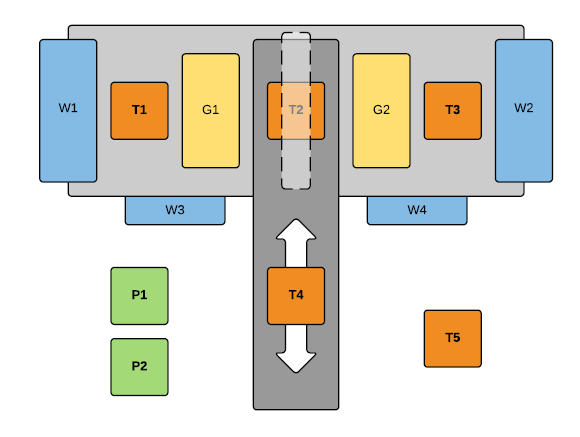
\includegraphics{wykresy/stanowisko.png}
\caption{Schemat stanowiska grzej�co-ch�odz�cego}
\label{stanowisko}
\end{figure}
\chapter{Zadanie 1: Punkt pracy}
Pierwszym poleceniem by�o okre�lenie warto�ci wyj�cia obiektu $Y_{pp}$ (pomiaru $T1$) w punkcie pracy $U_{pp} = 36$. Osi�gn�li�my j� ustawiaj�c warto�� sterowania (moc grzania grza�ki $G1$) na $U_{pp}$ i odczekuj�c znaczn� ilo�� czasu (powy�ej 5 minut). Jak wida� na wykresie \ref{pp}, wyj�cie ustabilizowa�o si� w okolicy 35 stopni Celcjusza. Jendak�e, z powodu narastaj�cej temperatury w ci�gu zaj��, punkt pracy zmienia� si�, nawet o ponad stopie� w g�r�, co b�dzie widoczne w nast�pnych zadaniach.


\begin{figure}[tb]
	\centering
	\begin{tikzpicture}
	\begin{axis}[
	legend pos=south east,
	width=0.9\textwidth,
	xmin=0,xmax=300,ymin=25,ymax=37,
	xlabel={$k$},
	ylabel={$S(k)$},
	xtick={0,50,100,150,200,250,300},
	ytick={25,26,27,28,29,30,31,32,33,34,35,36,37},
	y tick label style={/pgf/number format/1000 sep=},
	]
	\addplot[blue,semithick] file {wykresy/lab1U.txt};
	\addplot[red,semithick] file {wykresy/lab1Y.txt};
	
	\legend{$U$,$Y$}
	\end{axis}
	\end{tikzpicture}
	\caption{Zachowanie obiektu w punkcie pracy, $U_{pp}=\num{36}$}
	\label{pp}
\end{figure}
\FloatBarrier
\chapter{Zadanie 2: Odpowiedzi skokowe}
\section{Odpowiedzi skokowe}

W tej cz�ci projektu nale�a�o wyznaczy� symulacyjnie odpowiedzi skokowe (rys. \ref{odpskok}). Eksperyment zak�ada�, i� obiekt b�dzie na pocz�tku w punkcie pracy, a nast�pnie w chwili $k=15$ zostanie wykonany skok jednostkowy. 
\begin{figure}[tb]
	\centering
	\begin{tikzpicture}
	\begin{axis}[
	width=0.9\textwidth,
	height=0.3\textheight,
	xmin=0,xmax=150,ymin=-1,ymax=1,
	xlabel={$k$},
	ylabel={$U$},
	xtick={0,50,100,150},
	ytick={-1,-0.5,0,0.5,1},
	]
	\addplot[blue,semithick] file {wykresy/zad2/z2_u1.txt};
	\addplot[red,semithick] file {wykresy/zad2/z2_u4.txt};
	\addplot[green,semithick] file {wykresy/zad2/z2_u7.txt};
	\addplot[yellow,semithick] file {wykresy/zad2/z2_u10.txt};
	\addplot[brown,semithick] file {wykresy/zad2/z2_u13.txt};
	\addplot[orange,semithick] file {wykresy/zad2/z2_u16.txt};
	\addplot[magenta,semithick] file {wykresy/zad2/z2_u19.txt};
	\end{axis}
	\end{tikzpicture}
	\caption{Sterowanie}
	\label{uskok}
\end{figure}

\begin{figure}[tb]
	\centering
	\begin{tikzpicture}
	\begin{axis}[
	width=0.9\textwidth,
	height=0.3\textheight,
	xmin=0,xmax=200,ymin=-0.5,ymax=6,
	xlabel={$k$},
	ylabel={$Y$},
	xtick={0,50,100,150,200},
	ytick={-0.5,0,0.5,1,1.5,2,2.5,3,3.5,4,4.5,5,5.5,6},
	]
	\addplot[blue,semithick] file {wykresy/zad2/z2_y1.txt};
	\addplot[red,semithick] file {wykresy/zad2/z2_y4.txt};
	\addplot[green,semithick] file {wykresy/zad2/z2_y7.txt};
	\addplot[yellow,semithick] file {wykresy/zad2/z2_y10.txt};
	\addplot[brown,semithick] file {wykresy/zad2/z2_y13.txt};
	\addplot[orange,semithick] file {wykresy/zad2/z2_y16.txt};
	\addplot[magenta,semithick] file {wykresy/zad2/z2_y19.txt};
	\end{axis}
	\end{tikzpicture}
	\caption{Wyj�cie}
	\label{yskok}
\end{figure}


\section{Charakterystyka statyczna}
Poni�ej zosta�a zaprezentowana charakterystyka statyczna procesu $y(u)$ (rys. \ref{stat}).
Na podstawie zawartego wykresu mo�na wywnioskowa�, �e w�a�ciwo�ci statyczne procesu s� nieliniowe. 

\begin{figure}[tb]
	\centering
	\begin{tikzpicture}
	\begin{axis}[
	width=0.9\textwidth,
	height=0.5\textheight,
	xmin=-1,xmax=1,ymin=-0.5,ymax=6,
	xlabel={$U$},
	ylabel={$Y$},
	xtick={-1,-0.8,-0.6,-0.4,-0.2,0,0.2,0.4,0.6,0.8,1},
	ytick={-0.5,0,0.5,1,1.5,2,2.5,3,3.5,4,4.5,5,5.5,6},
	]
	\addplot[blue,semithick] file {wykresy/zad2/z2_stat.txt};
	\end{axis}
	\end{tikzpicture}
	\caption{Charakterystyka statyczna}
	\label{stat}
\end{figure}

\section{Charakterystyka dynamiczna}
Charakterystyka dynamiczna zosta�a wyznaczona zale�nie od wielko�ci skoku sterowania. Zmierzone zosta�o, po ilu krokach od momentu skoku r�nica warto�ci wyj�� obiektu i punktu pracy $Y_{pp}$ wynosi�a powy�ej $90\%$ ca�kowitego skoku warto�ci  wyj�� obiektu $Y(k)$. Z otrzymanych danych wynika, �e charakterystyka dynamiczna jest nieliniowa (rys. \ref{dynamiczna}).
\begin{figure}[tb]
	\centering
	\begin{tikzpicture}
	\begin{axis}[
	width=0.9\textwidth,
	height=0.5\textheight,
	xmin=-1,xmax=1,ymin=0,ymax=18,
	xlabel={$U$},
	ylabel={$Y$},
	xtick={-1,-0.8,-0.6,-0.4,-0.2,0,0.2,0.4,0.6,0.8,1},
	ytick={0,2,4,6,8,10,12,14,16,18},
	]
	\addplot[blue,semithick] file {wykresy/zad2/z2_dyn.txt};
	\end{axis}
	\end{tikzpicture}
	\caption{Charakterystyka dynamiczna}
	\label{dynamiczna}
\end{figure}
\chapter{Laboratorium: Zadanie 3: Znormalizowane odpowiedzi skokowe}
Kolejnym poleceniem by�o wyznaczy� znormalizowane odpowiedzi skokowe (takie jakie wymagane s� do algorytmu DMC) i zaproksymowa� je, u�ywaj�c w tym celu cz�onu inercyjnego drugiego rz�du z op�nieniem. Cz�on posiada 4 parametry: $T_1$, $T_2$, $K$ (dalej oznaczane jako $K_p$) i $T_d$ (w dalszej cz�ci sprawozdania oznaczane jako $TD$). Nazwy zosta�y zmienione, by nie myli� ich z parametrami algorytmu PID. Cz�on jest opisany wzorami powsta�ymi po przekszta�ceniu jego transmitancji:
\begin{equation}
\alpha_1=e^{-\frac{1}{T_1}}
\end{equation}
\begin{equation}
\alpha_2=e^{-\frac{1}{T_2}}
\end{equation}
\begin{equation}
a_1=-\alpha_1-\alpha_2
\end{equation}
\begin{equation}
a_1=\alpha_1\alpha_2
\end{equation}
\begin{equation}
b_1=\frac{K_p}{T_1-T_2}[T_1(1-\alpha_1)-T_2(1-\alpha_2)]
\end{equation}
\begin{equation}
b_1=\frac{K_p}{T_1-T_2}[\alpha_1T_2(1-\alpha_2)-\alpha_2T_1(1-\alpha_1)]
\end{equation}
\begin{equation}
y(k)=b_1u(k-TD-1)+b_2u(k-TD-2)-a_1y(k-1)-a_2y(k-2)
\end{equation}
\\
W celu doboru parametr�w cz�onu wykorzystano funkcj� fmincon. Jako pocz�tkowe warto�ci dobieranych parametr�w wybrali�my $[11,10,1,10]$, 11 i 10 dla $T_1$ i $T_2$, aby nie by�y takie same, 1 dla $K_p$, bo przy dotychczas zebranych przebiegach nie spodziewali�my si� du�ego wzmocnienia dla tego obiektu i 10 dla $TD$, bo z obserwacji wynika, �e op�nienie obiektu jest bliskie tej warto�ci. Od do�u ograniczyli�my wszystkie parametry zerami. Od g�ry ograniczyli�my je warto�ciami $[1000,1000,10,30]$, tak, by ka�dy parametr mia� przedzia� dostosowany do swoich potrzeb (du�e zmiany dla $T_1$ i $T_2$, ma�e zmiany dla $K_p$, $TD$ s�dz�c po wykresach nie powinno przekroczy� 30). 
\section{Wyb�r odpowiedzi skokowej}
�wiadomi faktu, �e dla obiektu nieliniowego, jakim jest stanowisko grzewcze, liniowy algotyrm DMC nie b�dzie dzia�a� optymalnie, postanowili�my przyj�� tak� odpowied�, �eby regulowa� poprawnie przynajmniej w dolnej cz�ci zakresu temperatur i cz�ciowo w jego g�rnej. Dlatego jako odpowied� do znormalizowania wybrali�my t� dla skoku o $dU = 15$, jako �e zawiera w sobie ca�y dolny zakres oraz niewielk� cz�� g�rnego. W wyniku normalizacji przekszta�cili�my j� do odpowiedzi jak� mieliby�my po skoku jednostkowym (odj�li�my od ka�dej zebranej pr�bki warto�� w punkcie pracy dla danego wyj�cia i podzielili�my otrzymane warto�ci przez skok). Nast�pnie po wykonaniu aproksymacji otrzymali�my parametry cz�onu r�wne $T_1 = 71,0271$, $T_2 = 5,2254$, $K_p = 0,3935$ i $Td = 13$ przy b��dzie optymalizacji $e = 0,0038$. Znormalizowan� odpowied� i jej aproksymacj� przedstawili�my na poni�szym wykresie \ref{norm_skoky}.

\begin{figure}[tb]
\centering
\begin{tikzpicture}
\begin{axis}[
width=0.9\textwidth,
xmin=0,xmax=300,ymin=0,ymax = 0.45,
xlabel={$k$},
ylabel={$S(k)$},
xtick={0,50,100,150,200,250,300,350},
ytick={0,0.1,0.2,0.3,0.4,0.5,0.6},
y tick label style={/pgf/number format/1000 sep=},
legend pos=south east,
]
\addplot[blue,semithick] file {wykresy/lab3_15.txt}; 
\addplot[orange,semithick] file{wykresy/aprskok15.txt};

\legend{odpowied� skokowa,aproksymacja}
\end{axis}
\end{tikzpicture}
\caption{Wykres znormalizowanej odpowiedzi skokowej i jej aproksymacji}
\label{norm_skoky}
\end{figure}

\end{document}


